\section{Introduction}
\label{sec:intro}

%\jure{The paper is great! It reads very nicely and is very thoroughly and accurately written. Great job!! I left quite some comments but don't worry about them. They are all optional. :) }

%\jure{ Here are a few high-level comments and observations:\\
%1) Method is described very densely and it takes quite a bit of staring at the paper and connecting different parts to get what is going on. I would suggest taking a bit more space and being a bit more verbose in the method description.\\
%2) Experiments are extensive but some parts feel like a bit too much detail (hyperparameters, baseline settings, etc.). I think we can move those details to the supp materials and then use this space to expand on the method.\\
%3) When we describe experimental results, let's say "PHIL outperfosm method X by 40\% on average". Let's quantify and summarize the performance improvement. Saying "PHIL wins everywhere except in this one case" is actually putting emphasis on the one case rather than to put emphasis on how great our method is.\\}

Search heuristics are essential in several domains, including robotics, AI, biology, and chemistry \cite{bhardwaj2017learning, chen2020retro, gebser2013domain, mac2016heuristic, sharma2017identifying, yeh2012pathway}. For example, in robotics, complex robot geometries often yield slow collision checks, and search algorithms are constrained by the robot's onboard computation resources, requiring well-performing search heuristics that visit as few nodes as possible~\cite{bhardwaj2017learning, mac2016heuristic}. In AI, domain-specific search heuristics are useful for improving the performance of inference engines operating on knowledge bases \cite{gebser2013domain, sharma2017identifying}. Search heuristics have been previously also developed to reduce search efforts in protein-protein interaction networks \cite{yeh2012pathway} and in planning chemical reactions that can synthesize target chemical products \cite{chen2020retro}. This broad set of applications underlines the importance of good search heuristics that are applicable to a wide range of problems. 


%\jure{Number of examples here is long, perhaps we can cut one or two to save space.} \update{Removed game dev and b\&b}


%We formulate finding search heuristics as an optimization process, allowing practitioners to quickly find useful search heuristics. We illustrate this concept in Figure \ref{fig:money-fig}.

\begin{figure}[!htpb]
\centering
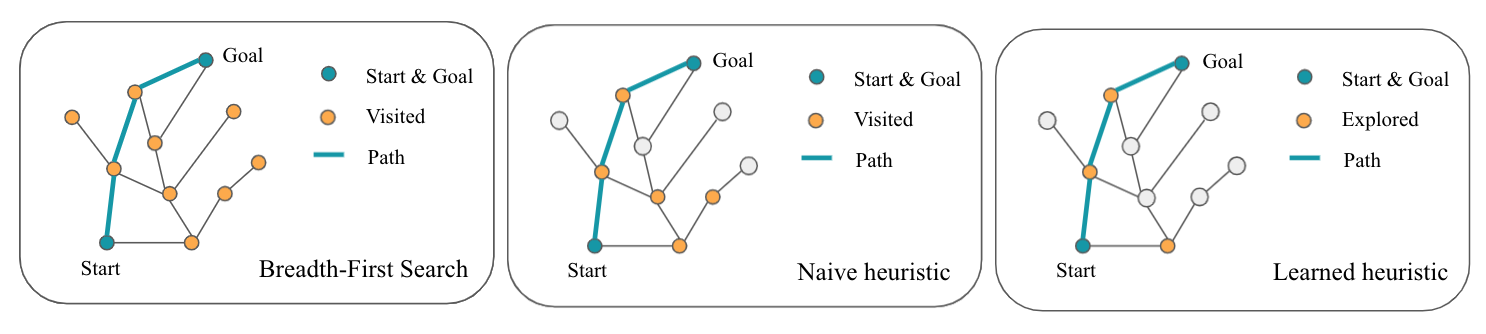
\includegraphics[width=0.9\textwidth]{figures/money_fig.png}
\caption{The goal is to navigate (find a path) from the start to the goal node. While BFS visits many nodes to find a start-to-goal path (left), one can use a heuristic based on the features of the nodes (e.g., Euclidean distance) on the graph to reduce the search effort (middle). We propose \alg to learn a tailored search heuristic for a given graph, capable of reducing the number of visited nodes even further by exploiting the inductive biases of the graph (right). }
\label{fig:money-fig}
\end{figure}

The search task can be formulated as a pathfinding problem on a graph, where given a graph, the task is to navigate and find a short feasible path from a start node to a goal node, while in the process visiting as few nodes as possible (Figure~\ref{fig:money-fig}). The most straightforward approach would be to launch a search algorithm such as breadth-first search (BFS) and iteratively expand the graph from the start node until it reaches the goal node. Since BFS does not harness any prior knowledge about the graph, it usually visits many nodes before reaching the goal, which is expensive in cases such as robotics where visiting nodes is costly. To visit fewer nodes during the search, one may use domain-specific information about the graph via a \textit{heuristic} function \cite{pearl1984heuristics}, which allows one to define a distance metric on graph nodes to prune directions that seem less promising to explore. Unfortunately, coming up with good search heuristics requires significant domain expertise and manual effort.
%, without straightforward ways to further refine proposed heuristics. 

While there has been significant progress in designing search heuristics, it remains a challenging problem. Classical approaches \cite{khalidi2020t, adabala2020multi} tend to hand-design search heuristics, which requires domain knowledge and a lot of trial and error. To alleviate this problem, there has been significant development in general-purpose search heuristics based on trading-off greedy expansions and novelty-based exploration \cite{xie2012planning, xie2014adding, lipovetzky2017best, teichteil2021boundary} or search problem simplifications \cite{bonet2001planning, zhu2003landmark, richter2010lama}. These approaches alleviate some of the common pitfalls of goal-directed heuristics, but we demonstrate that if possible, it is useful to learn domain-specific heuristics that can better exploit problem structure.

On the other hand, learning-based methods face a set of different challenges. Firstly, the data distribution is not i.i.d., as newly encountered graph nodes depend on past heuristic values, which means that supervised learning-based methods are not directly applicable. Secondly, heuristics should run fast, with ideally constant time complexity. Otherwise, the overall asymptotic time complexity of the search procedure could be increased. Finally, as the environment (search graph) sizes increase, reinforcement learning-based heuristic learning approaches tend to perform poorly \cite{bhardwaj2017learning}. State-of-the-art imitation learning-based methods can learn useful search heuristics \cite{bhardwaj2017learning}; however, these methods still rely on feature-engineering for a specific domain and do not generally guarantee a constant time complexity with respect to graph sizes.


\begin{figure}[h]
\centering
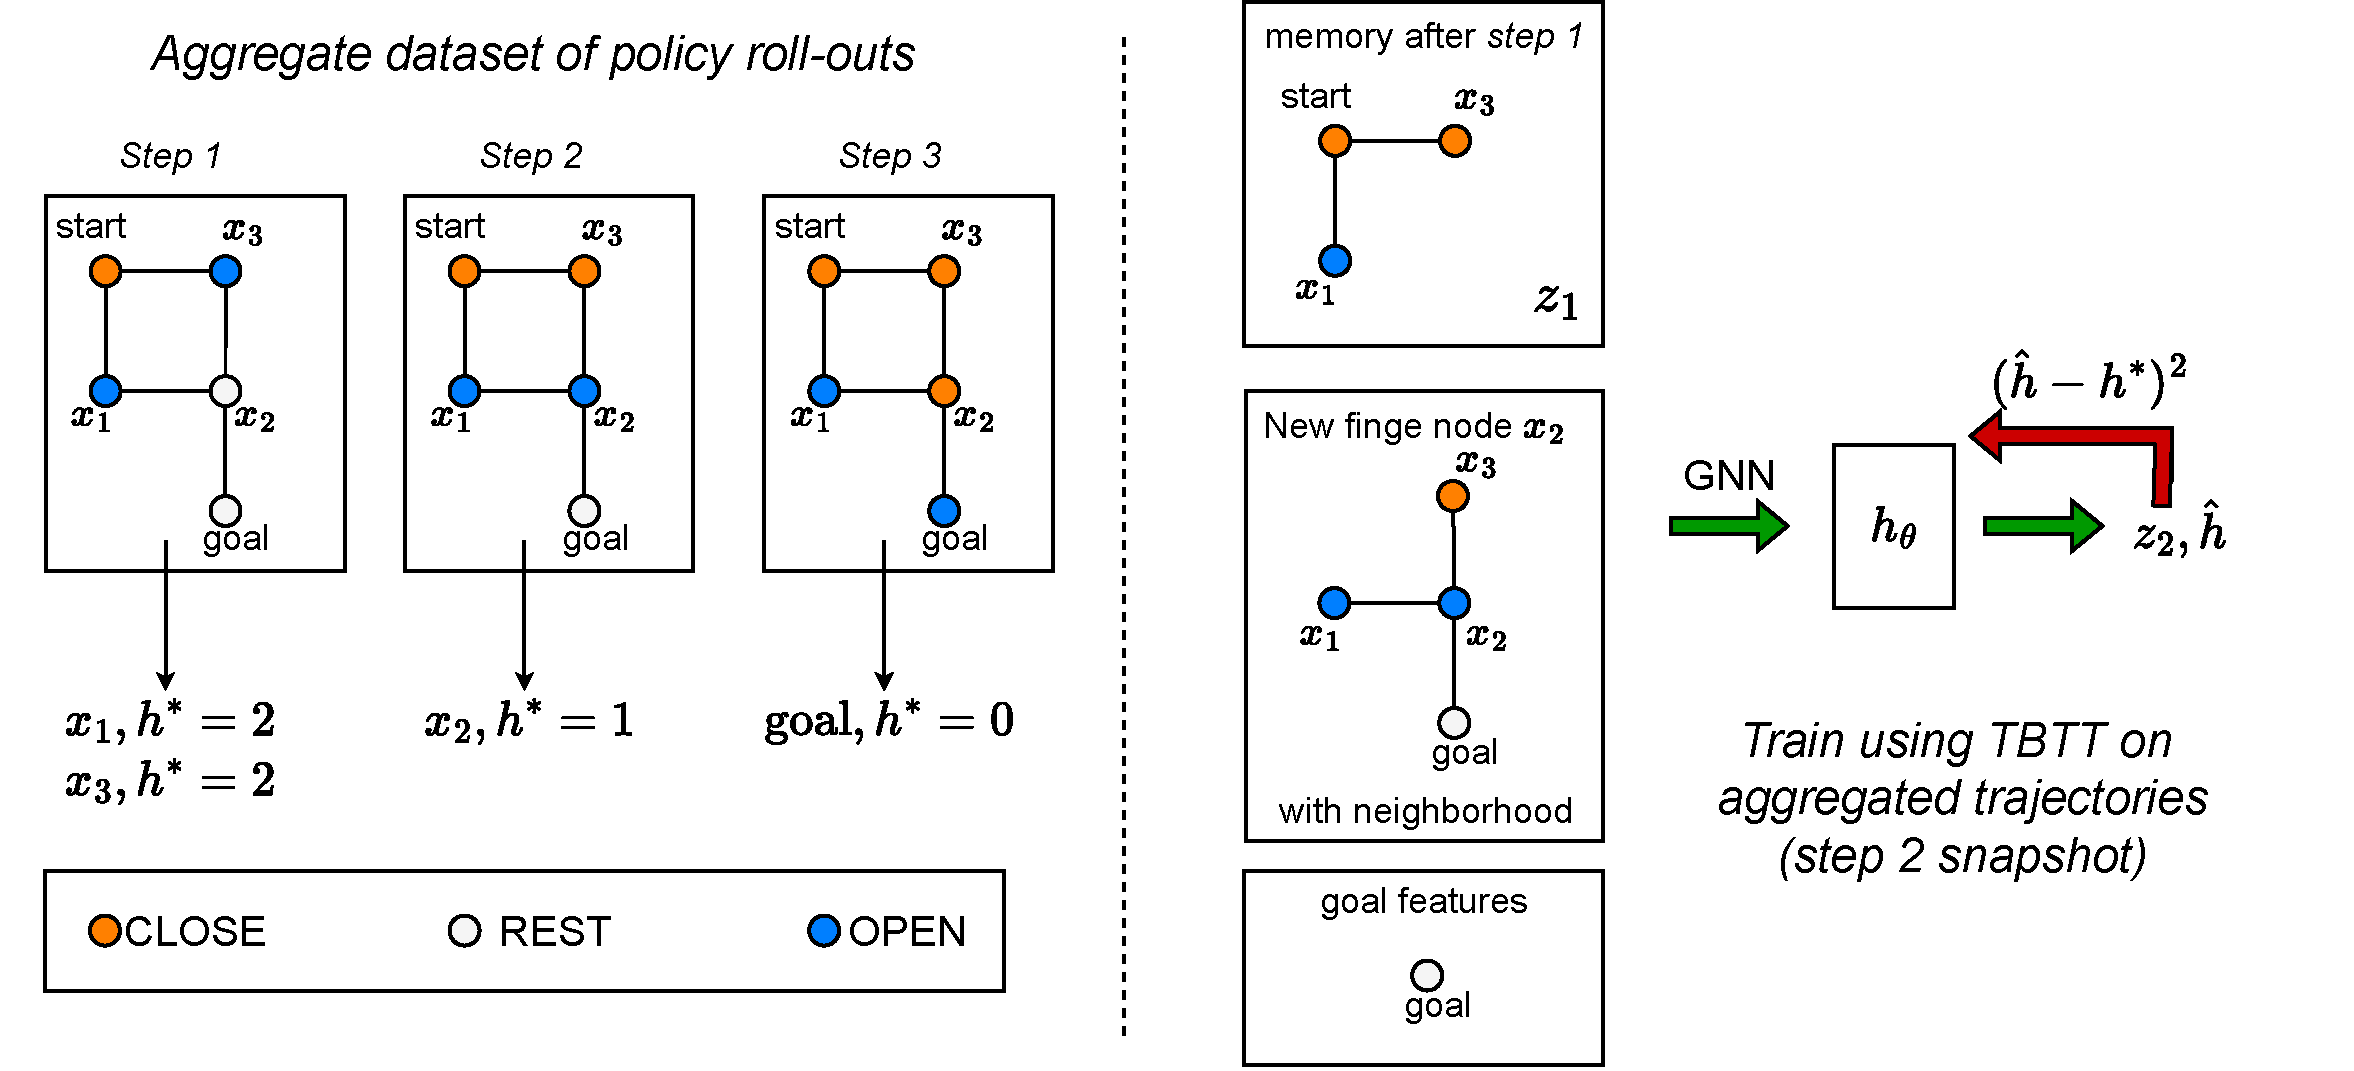
\includegraphics[width=0.9\textwidth]{figures/method_figure2.pdf}
\caption{Main components of \alg: On the left, using a greedy mixture policy induced by the current version of our parameterized heuristic $h_\theta$ and an oracle heuristic $h^*$ (i.e., a heuristic that correctly determines distances between nodes), we roll-out a search trajectory from the start node to the goal node. Each trajectory step contains a set of newly added fringe nodes with bounded random subsets of their 1-hop neighborhoods and their oracle ($h^*$) distances to the goal node. Trajectories are aggregated throughout the training procedure. On the right, we use truncated backpropagation through time on each collected trajectory to train $h_\theta$, where $\hat{h}$ is the predicted distance between $x_2$ and $x_g$, and $z_2$ is the updated state of the memory. Here, the memory captures the embedding of the graph visited so far.}
\label{fig:approach-high-level}
\end{figure}

%\jure{Here we say ``memory'', can we continue the sentence to explain what memory is. Something like: , which captures the graph visited so far.} \update{Added a short sentence at the end}
%\jure{Questions:\\
%-- what is "aggregate dataset"? So far we just explained that there is a graph, a start and a goal node. We need to explain what "aggregate dataset" is or change the label.\\
%-- can we use the concepts introduce in the main text in this figure as well.\\
%-- why do we label $x_{end}$? shouldn't we call it $x_{g}$. Let's use consistent terminology. Also $d_gt$ can we define it.\\
%-- Basically, if we use symbols in the figure, let's define them in the caption.}

%We formulate finding search heuristics as an optimization process, allowing practitioners to quickly find useful search heuristics. We illustrate this concept in Figure \ref{fig:money-fig}.


In this paper, we propose \textit{Path Heuristic with Imitation Learning} (\alg), a framework that extends the recent imitation learning-based heuristic search paradigm with a learnable \textit{explored graph memory}. This means that \alg learns a representation that allows it to capture the structure of the so far explored graph, so that it can then better select what node to explore next (Figure \ref{fig:approach-high-level}).  We train our approach to predict the node-to-goal distances ($h^{*}$ in Figure \ref{fig:approach-high-level}) of graph nodes during search. To train our memory module, which captures the explored graph, we use truncated backpropagation through time (TBTT) \cite{sutskever2013training}, where we utilize ground-truth node-to-goal distances as a supervision signal at each search step. Our TBTT procedure is embedded within an adaptation of the AggreVaTe imitation learning algorithm \cite{ross2014reinforcement}. \alg also includes a \textit{specialized graph neural network architecture}, which allows us to apply \alg to diverse graphs from different domains.

%\jure{Here we introduce many concepts: like ``explored graph'', ``memory module'', ``TBTT'', ``cost-to-go'', ... Can we please make sure to use these concepts in Fig 2 (have some part of the figure labeled using these labels.}

%Figure \ref{fig:approach-high-level} presents the high-level idea of our approach. 

We evaluate \alg on standard benchmark heuristic learning datasets (Section \ref{sec:experiments-grids}), diverse graph-based datasets from different domains (Section \ref{sec:experiments-diversity}), and practical UAV flight use cases (Section \ref{sec:experiments-drone}). Experiments demonstrate that \alg outperforms state-of-the-art heuristic learning methods up to $4 \times$. Further, \alg performs within $4.9 \%$ of an oracle in indoor drone planning scenarios, which is up to a $21.5 \%$ reduction compared with commonly used approaches. In practice, our contributions enable practitioners to quickly extract useful search heuristics from their graph datasets without any hand-engineering.